\chapter{Διάλογος και Συστάσεις}

Σε αυτό το κεφάλαιο θα περιγράψουμε πολύ περιληπτικά την χρήση της ενισχυτικής μάθησης σε διαλογικά συστήματα, ώστε να μπορέσουμε να το συνδέσουμε με το πρόβλημα μας, και μετά θα περιγράψουμε την χρήση ενισχυτικής μάθησης σε προβλήματα συστάσεων, που είναι και πιο κοντά στο πεδίο του προβλήματος μας.

\section{Διάλογικά Συστήματα}

Η ιδέα της δημιουργίας ενός πράκτορα που θα μπορεί να απαντήσει σε ανθρώπινες ερωτήσεις, ξεκίνησε από το σύγγραμα του \en{Alan Turing, Computing Machinery and Intelligence} \cite{turing1950computing}. Τα πρώτα μοντέλα που δημιουργήθηκαν βασίζονταν σε κανόνες, όπου αναγνώριζαν κάποιες λέξεις-κλειδία στο κείμενο και ανάλογα με αυτές απαντούσαν στον χρήστη. Το πρόβλημα αυτών των συστημάτων ήταν ότι ήταν πολύ δύσκολο να επεκταθούν, καθώς και να γενικεύσουν, αφού η δημιουργοί πρέπει να προσθέσουν χειροκίνητα τους επιπλέον κανόνες. Τα τελευταία χρόνια, η δημιουργία διαλογικών συστημάτων γίνεται ολοένα και περισσότερο με χρήση βαθειάς μηχανικής μάθησης, παρόλο που η χρήση κανόνων είναι ακόμα βολική σε κάποιες περιπτώσεις.

Tα διαλογικά συστήματα συνήθως χωρίζονται σε δύο κατηγορίες ανάλογα με τον σκοπό τους:
\begin{enumerate}
    \item Συγκεκριμένου σκοπού (\en{task-oriented systems}). Τα διαλογικά αυτά συστήματα έχουν ως στόχο να βοηθήσουν τον χρήστη να πετύχει συγκεκριμένους στόχους, ιδανικά σε όσο λιγότερους γύρους διαλόγου γίνεται. Για παράδειγμα τέτοια συστήματα είναι συστήματα μέσω των οποίων ο χρήστης μπορεί να κλείσει εισητήρια, ή να λάβει υποστήριξη σχετικά με ένα πρόβλημα του.
    \item Ανοιχτού σκοπού (\en{open-domain systems}). Τα διαλογικά συστήματα αυτά δεν έχουν κάποιο σκοπό, αλλά εστιάζουν στο να δώσουν ρεαλιστικές απαντήσεις σε συζητήσεις με τον χρήστη. 
\end{enumerate}

\begin{figure}
    \centering
    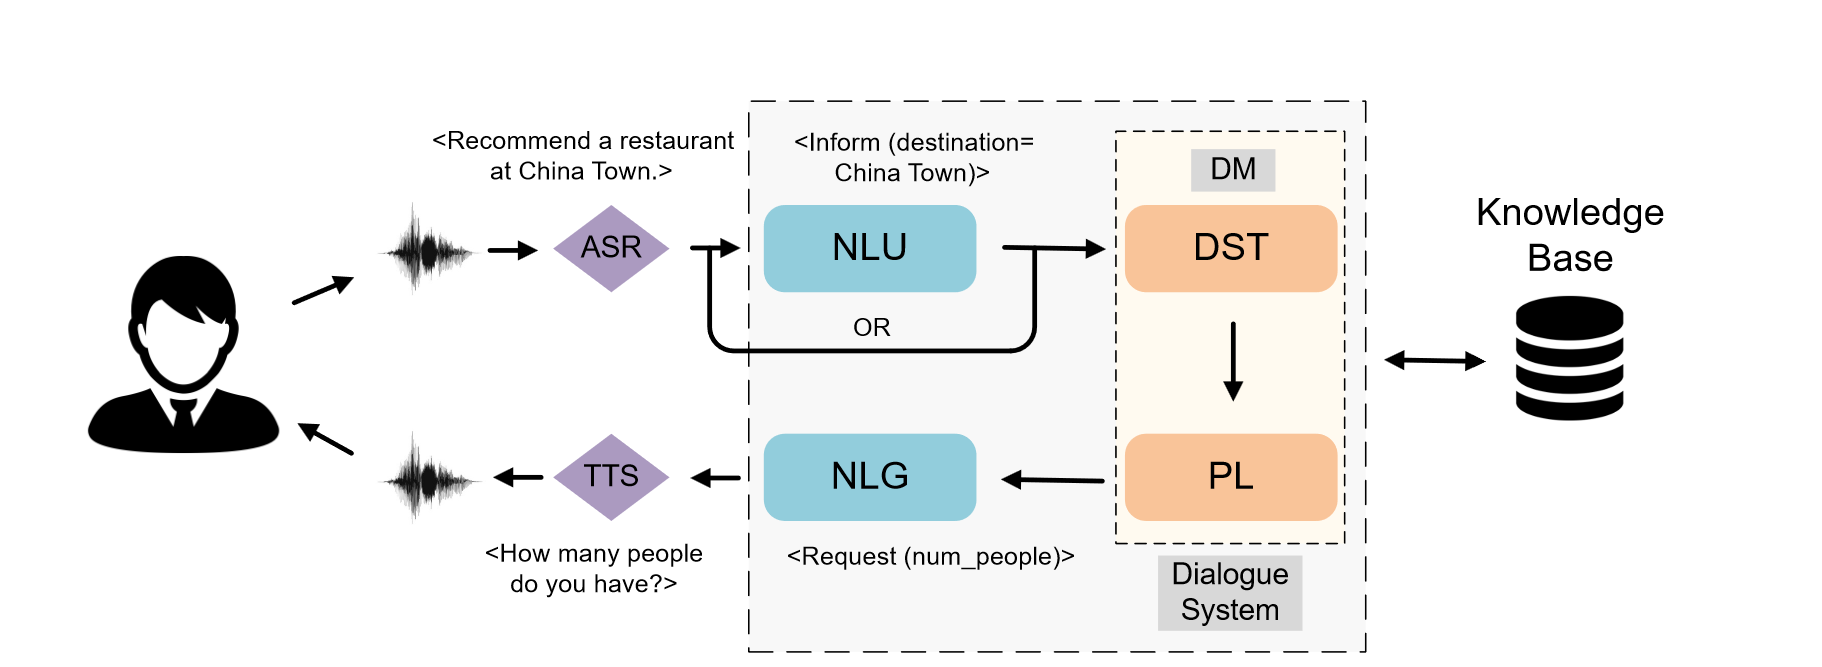
\includegraphics[width=\textwidth]{body_matter/dialogue_and_recommendations/images/task-based-dialogue-system.png}
    \caption{Σύστημα συγκεκριμένου σκοπού \cite{recent_advances_dl_2021}}
    \label{fig:task_based_system}
\end{figure}

Συχνά τα συστήματα συγκεκριμένου σκοπού οργανώνονται σε μια αλληλουχία μερών όπως αυτή που φαίνεται στο Σχήμα~\ref{fig:task_based_system}:
\begin{itemize}
    \item \textbf{Το κομμάτι της κατανόησης της εισόδου του χρήστη.} Αυτό το κομμάτι είνα υπευθυνο για την ταξινόμηση των διάφορων λέξεων σε μέρη του λόγου, την αναγνώριση ονομάτων, αλλά και την αναγνώριση της πρόθεσης του χρήστη με βάση το τι είπε. Κάποια συστήματα δεν χρησιμοποιούν αυτό το κομμάτι και χρησιμοποιούν το ίδιο το μήνυμα του χρήστη ως είσοδο στο επόμενο κομμάτι, όπως στο Σχήμα~\ref{fig:task_based_system}. Αυτό συμβαίνει για να μειώσουν την επίδραση του λάθους του πρώτου αυτού του κομματιού και την μεταφορά λαθών στα μετέπειτα κομμάτια. 
    \item \textbf{Το κομμάτι της διαχείρισης της κατάστασης του διαλόγου,} το οποίο ρυθμίζει τις καταστάσεις του διαλόγου με βάση την τρέχουσα είσοδο και την ιστορία του διαλόγου. Η κατάσταση του διαλόγου περιέχει σχετικές δράσεις του χρήστη και ζευγάρια θέσης-τιμής. 
    \item \textbf{Το κομμάτι της εκμάθησης της πολιτικής του διαλόγου}, το οποίο με βάση τις καταστάσεις του διαλόγου που παίρνει από το προηγούμενο κομμάτι, επιλέγει την επόμενη δράση του διαλογικού πράκτορα.
    \item \textbf{Το κομμάτι της παραγωγής της απάντησης του συστήματος}, το οποίο μετατρέπει τις δράσεις που επιλέχθηκαν από το προηγούμενο κομμάτι σε φυσική γλώσσα, η οποία θα επιστραφεί στον χρήστη. 
\end{itemize}

Άλλες φορές προτιμάται ένα σύστημα που υλοποιεί όλες τις παραπάνω λειτουργίες από άκρη σε άκρη, το οποίο μπορεί να πετύχει καλύτερη βελτιστοποίηση, καθώς δεν υπάρχει μεταφορά σφάλματος μεταξύ των διάφορων κομματιών.

\subsection{Ενισχυτική Μάθηση και Διαλογικά Συστήματα}

Όσον αφορά την χρήση ενισχυτικής μάθησης, σε συστήματα συγκεκριμένου σκοπού είναι στην διαχείρηση του διαλόγου. Πιο συγκεκριμένα δύο σύνηθεις χρήσεις είναι για την παρακολούθηση της κατάστασης του διαλόγου και την εκμάθηση της πολιτικής. Η δεύτερη χρήση είναι ιδιαίτερα σύνηθης και αρκετά επιτυχημένη, καθώς περιγράφεται ακριβώς από ένα πρόβλημα ΕΜ (πχ \cite{policy_learning_2019}). 

Σε συστήματα ανοιχτού σκοπού, η χρήση της ενισχυτικής μάθησης είναι κυρίως η επιλογή απαντήσεων παρά η παραγωγή τους, καθώς τα παραγωγικά \en{generative} συστήματα είναι πολύ καλύτερα στην παραγωγή λόγου. 

Για παράδειγμα, σε μια από τις πρώτες δουλείες οι οποίες χρησιμοποιήσαν ΕΜ σε διάλογο \cite{rl_dialogue_2016}, οι συγγραφείς προσπάθησαν να ενώσουν τις ιδέες από τα \en{seq2seq} μοντέλα και την ΕΜ, ώστε να δημιουργήσουν συστήματα τα οποία επιστρέφουν καλύτερες απαντήσεις. Έτσι δημιούργησαν μια μετρική ανταμοιβής η οποία αξιολογούσε την ποιότητα των απαντήσεων. Αρχικά εκπαίδευσαν ένα \en{seq2seq} μοντέλο με επιβλεπόμενη μάθεση, και μετά με βάση αυτό προσομοιώσαν διαλόγους μεταξύ δυο πρακτόρων, ξεκινώντας από μια πρόταση από το σύνολο εκπαίδευσης.

Ενα από τα πιο διάσημα σύχρονα παραδείγματα είναι η χρήση του στην εκπαίδευση του \en{InstructGPT}. Στο \cite{chatgpt_2022}, οι ερευνητές έκαναν \en{fine-tune} το {GPT-3} με χρήση ενισχυτικής μάθησης και ανατροφοδότησης από ανθρώπους. Συγκεκριμένα, κατα το \en{fine-tuning}, το μοντέλο "ρώταγε" τους χρήστες ποιά από τις απαντήσεις θεωρούσαν καλύτερη σε σχέση με ένα ερώτημα, οι χρήστες ταξινομούσαν τις απαντήσεις από καλύτερη προς χειρότερη, και με βάση αυτό εκπαιδεύτηκε ένα μοντέλο ανταμοιβών. Έπειτα, για την εκπαίδευση της πολιτικής των απαντήσεων του συστήματος, ενα ερώτημα επιλεγόταν από το σύνολο των δεδομένων, η πολιτική του συστήματος παράγει μια έξοδο και το μοντέλο ανταμοιβών επιλέγει την ανταμοιβή για αυτή την έξοδο. Με βάση αυτό ανανεώνεται η ανταμοβή της πολιτικής. 

\section{Συστήματα Συστάσεων}

Ένα σύστημα συστάσεων αποτελείται από εργαλεία και αλγορίθμους οι οποίοι αναπτύχθηκαν με την ιδέα να βοηθήσουν τους χρήστες να βρουν αντικείμενα που τους ενδιαφέρουν. Σε μια γενική μορφή, ο στόχος είναι η δημιουργία του προφίλ των χρηστών βασισμένη στην ανατροφοδότηση μεταξύ συστήματος και χρήστη και η σύσταση αντικειμένων που να ταιριάζουν στο προφίλ αυτό. Το πρόβλημα απαντάται σε πολλούς κλάδους όπως της υγείας, της διασκέδασης, των νέων, κλπ.

Παραδοσιακά το πρόβλημα των συστάσεων θεωρούνταν ένα πρόβλημα ταξινόμησης ή πρόβλεψης, αλλά πλεον ο ακαδημαικός κόσμος συμφωνεί ότι η αλληλεπίδραση μεταξύ χρήστη και συστήματος μοντελοποιήται καλύτερα ως ενα πρόβλημα αποφάσεων με διαδοχικά βήματα \cite{rl_recommenders_2021}. Έτσι μπορεί να περιγραφεί από μια Μαρκοβιανή Διαδικασία Αποφάσεων και να λυθεί με χρήση ενισχυτικής μάθησης.

Πρωτού περάσουμε σε τεχνικές με χρήση ενισχυτικής μάθησης, είναι σημαντικό να γνωρίσουμε περιληπτικά τους κλασικούς αλγορίθμους. Αυτόι είναι:
\begin{itemize}
    \item \textit{Συνεργατικό φιλτράρισμα}: Η ιδέα της μεθόδου είναι η ομαδοποίηση του χρήστη (ή των αντικειμένων) σε ομάδες με παρόμοια χαρακτηριστικά. Όταν το φιλτράρισμα γίνεται με βάση τον χρήστη, οι προτάσεις γίνονται με βάση τις παρόμοιες προτιμήσεις διάφορων χρηστών. Από την άλλη, όταν αναφερόμαστε σε φιλτράρισμα με βάση τα αντικείμενα, οι προτάσεις γίνονται με βάση τα αντικείμενα τα οποία σχετίζονται με αυτά που ο χρήστης έχει ήδη αλληλεπιδράσει. Η μέθοδος αυτή μπορεί να χωριστεί σε δύο προσεγγίσεις: με βάση την μνήμη, όπου ουσιαστικά για κάθε χρήστη/αντικείμενο γίνεται μια σύγκριση ομοιότητας (πχ ομοιότητα συνημιτόνου) με τους υπόλοιπους και μετά με χρήση $k$-κοντινότερων γειτόνων, ή με βάση κάποιο μοντέλο, όπου ουσιαστικά δημιουργήται ένα μοντέλο που εκπαιδεύεται με τεχνικής μηχανικής μάθησης να βρίσκει ομοιότητες μεταξύ χρήστες \cite{7872755}.
    \item \textit{Παραγοντοποίηση πινάκων}: Αυτή η μέθοδος χρησιμοποιήται και ξεχωριστά και ως μέρος του φιλτραρίσματος. Η ιδέα είναι η αναπαράστααση του χρήστη και των αντικειμένων ως αντικείμενα σε ένα χώρο λίγων διαστάσεων. Έπειτη η συμβατότητα χρήστη και προιόντος υπολογίζεται είτε με χρήση εσωτερικού γινομένου, ή με χρήση κάποιου νευρωνικού δικτύου αν οι σχέσει είναι μη γραμμικές. 

Οι κλασικές μέθοδοι, έχουν διάφορα προβλήματα, όπως το ότι το σύστημα δεν μπορεί να προσφέρει χρήσιμες συστάσεις σε ένα νέο χρήστη, ή οταν προστίθεται ένα νέο αντικείμενο (\en{cold-start}), ενώ δεν μπορεί να κλιμακώσει, να ανταπεξέλθει σε ποικιλία, έχει χαμηλής ποιότητας προτάσεις, και είναι υπολογιστικά ακριβά \cite{jannach_zanker_felfernig_friedrich_2010}.

Μια άλλη προσέγγιση στις συστάσεις είναι μέσω χρήσης βαθειάς μάθησης, όμως είναι δύσκολο να καταλάβουμε πως δουλεύουν αυτά τα μοντέλα και χρειάζονται πάρα πολλά δεδομένα και υπολογισμούς για να κάνουν καλές προβλέψεις.

Σε αντίθεση με τις κλασικές μεθόδους, η ΕΜ μπορεί να διαχειριστεί ακολουθιακές και δυναμικές αλληλεπιδράσεις μεταξύ συστήματος και χρήστη και να λάβει υπ'όψιν την μακροχρόνια αφοσίωση των χρηστών. 

Η χρήση \en{contextual bandits} για 


\end{itemize}